
\textbf{Ejemplo 2}\\
Un inversionista en Colombia adquiere un documento que vale 300 US, gana un
interés del 6\% nominal anual año vencido en dólares a un plazo de un año. El
tipo de cambio actual es  1 US =  1.500 COP y se estima una devaluación del peso con respecto al dólar durante ese año del 20\% efectivo anual. Calcular la rentabilidad que se podía obtener. ¿Cuál es la rentabilidad neta, una vez descontada la retención en la fuente del 7\%?\\ \\
%\newpage %USAR SOLO SI EL SOLUCIÓN QUEDA SOLO Y ES NECESARIO BAJARLO A LA SIGUIENTE PAGINA
\textbf{Solución.}\\
%La tabla ira centrada
\begin{center}
 \renewcommand{\arraystretch}{1.5}% Margenes de las celdas
 %Creación de la cuadricula de 3 columnas
 \begin{longtable}[H]{|c|c|c|}
  %Creamos una linea horizontal
  \hline
  %Definimos el color de la primera fila
  \rowcolor[HTML]{FFB183}
  %%%%% INICIO DECLARACIÓN DE VARIABLES %%%%%%%
  %%%%%%%%%% INICIO TITULO
  %Lo que se hace aquí es mezclar las 3 columnas en una sola
\multicolumn{3}{|c|}{\cellcolor[HTML]{FFB183}\textbf{1. Asignación de Periodo Focal}}                                        \\ \hline
  %%%%%%%%%% FIN TITULO
  %%%%%%%%%% INICIO DE MATEMÁTICAS
  %Cada & hace referencia al paso de la siguiente columna
  \multicolumn{3}{|c|}{\textit{$pf = 1 pav$}}                                                            \\ \hline
  \multicolumn{3}{|c|}{\cellcolor[HTML]{FFB183}\textbf{2. Declaración de variables}}                                        \\ \hline
  %%%%%%%%%% FIN TITULO
  %%%%%%%%%% INICIO DE MATEMÁTICAS
  %Cada & hace referencia al paso de la siguiente columna
  $j = 6\% \textit{ naav en US}$                                     & $n = 1 \textit{ pav} $ & $j_{dev}=20\% \textit{ naav}$ \\
  $i = \frac{6 \textit{ naav}}{1 \textit{ pav}} = 6\% \textit{ pav}$ & dólar:1 US = $ 1.500 \ COP $  &                             \\ \hline

  %%%%%%%%%% FIN DE MATEMÁTICAS
  %%%%% FIN DECLARACIÓN DE VARIABLES


  %%%%% INICIO FLUJO DE CAJA
  \rowcolor[HTML]{FFB183}
  \multicolumn{3}{|c|}{\cellcolor[HTML]{FFB183}\textbf{3. Diagrama de flujo de caja}}                                       \\ \hline
  %Mezclamos 3 columnas y pondremos el dibujo
  %%%%%%%%%%%%% INSERCIÓN DE LA IMAGEN
  %Deberán descargar las imágenes respectivas del drive y pegarlas en la carpeta
  %n_capitulo/img/ejemplos/1/capitulo1ejemplo1.pdf  (el /1/ es el numero del ejemplo)
  \multicolumn{3}{|c|}{ 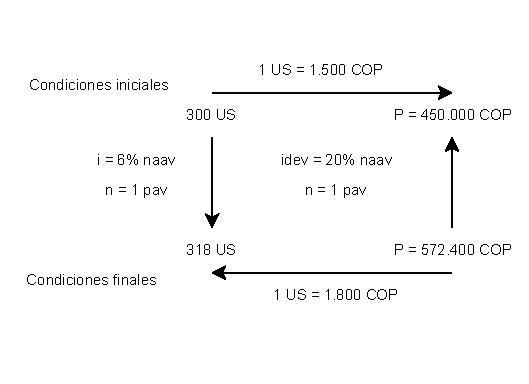
\includegraphics[trim=-78 -5 -78 -5]{3_Capitulo/img/ejemplos/2/capitulo3ejercicio2.pdf} }                         \\ \hline
  %%%%%%%%%%%%% FIN INSERCIÓN DE IMAGEN
  %%%%%FIN FLUJO DE CAJA



  %%%%% INICIO DECLARACIÓN FORMULAS
  %%%%%%%%%%% INICIO TITULO
  \rowcolor[HTML]{FFB183}
  \multicolumn{3}{|c|}{\cellcolor[HTML]{FFB183}\textbf{4. Declaración de Fórmulas}}                                         \\ \hline
  %%%%%%%%%%% FIN TITULO
  %%%%%%%%%%% INICIO MATEMÁTICAS
  \multicolumn{3}{|c|}{$F = P (1 + i)^n \textit{ Valor futuro}$}                                                            \\ \hline
  %%%%%%%%%% FIN MATEMÁTICAS
  %%%%%% INICIO DESARROLLO MATEMÁTICO
  \rowcolor[HTML]{FFB183}
  %%%%%%%%%%INICIO TITULO
  \multicolumn{3}{|c|}{\cellcolor[HTML]{FFB183}\textbf{5. Desarrollo Matemático}}                                           \\ \hline
  %%%%%%%%%% FIN TITULO
  %%%%%%%%%% INICIO MATEMÁTICAS
    \multicolumn{3}{|p{\textwidth}|}{
  $300 \ US$ en pesos, $(300)1{.}500 =  450{.}000 \ COP$ \vspace{3mm} \newline

  $F = 300 \ US(1 + 0,06)1 = 318 \ US$ \vspace{3mm} \newline

  $F =  1{.}500 \ COP (1 + 0,02)^1=  1{.}800 \ COP$\newline

  $  (318 \ US)\frac{ 1{.}800 \ COP}{1 \ US}= 572{.}400 \ COP$\newline

  $ \frac{(318 US \  COP) 1{.}800 \ COP}{ 1 \ US} =  572{.}400 \ COP$ \newline
  }                                                                                                                         \\ \hline
\multicolumn{3}{|c|}{\cellcolor[HTML]{FFB183}\textbf{6. Respuesta}}                                         \\ \hline
  %%%%%%%%%%% FIN TITULO
  %%%%%%%%%%% INICIO MATEMÁTICAS
\multicolumn{3}{|p{\textwidth}|}{El valor de la rentabilidad sin descontar la retención en la fuente era de 572.400 COP con un i del 27,2\%. Al descontar la retención en la fuente esa rentabilidad neta es de
563,832 COP, con un i del 25\%}  \\ \hline
  %%%%%%%%%% FIN MATEMÁTICAS

  %%%%%%%%%% FIN MATEMÁTICAS
  %%%%%% FIN DESARROLLO MATEMÁTICO
  %%%%%% INICIO RESPUESTA



  %%%%%%%%%% FIN MATEMÁTICAS
  %%%%%% FIN RESPUESTA
 \end{longtable}
 %Se crean dos lineas en blanco para que no quede el siguiente texto tan pegado
 %\newline \newline %USARLO SI CREES QUE ES NECESARIO
\end{center}